\chapter{一元随机变量概述}
\begin{introduction}
  \item Intro to Prob\quad2.1
  \item Prob $\&$ Stat\quad2.1
\end{introduction}
\section{随机变量的定义}

\begin{definition}{随机变量} \label{def: random_variable} 
定义在样本空间 $\Omega$ 上的 {\textbf 实值函数} $X=X(\omega),\omega \in \Omega$,称$X$为随机变量。
\end{definition}
\begin{remark}
通常用大写字母$X,Y,Z$表示随机变量,其取值用小写字母$x,y,z$等表示。
\end{remark}

\begin{example}
考虑抛一枚硬币三次的结果。记硬币正面朝上为“1”,而硬币反面朝上为“0”。我们考虑样本空间及硬币正面朝上的次数。
\begin{table}[ht]
  \centering
  \caption{抛三枚硬币的结果}\label{tab:Lect3_3coins}
  \begin{tabular}{cc}
    \toprule
    抛三次硬币的结果 & 正面朝上的次数$X$ \\
    \midrule
    $\omega_1$ = (反,反,反) & 0\\
    $\omega_2$ = (正,反,反) & 1\\
    $\omega_3$ = (反,正,反) & 1\\
    $\omega_4$ = (反,反,正) & 1\\
    $\omega_5$ = (正,正,反) & 2\\
    $\omega_6$ = (正,反,正) & 2\\
    $\omega_7$ = (反,正,正) & 2\\
    $\omega_8$ = (正,正,正) & 3\\
    \bottomrule
  \end{tabular}
\end{table}

这里,一枚硬币抛三次,正面朝上的次数就是所定义的{\textbf{随机变量}}。
\end{example}

\begin{remark}
总结如下:
    \begin{enumerate}
    \item 不同的样本点对应不同的实数;
    \item 多个样本点对应同一个实数;
    \item 样本点可以用数值表示,也可以不用数值表示;但随机变量一定是数值型。
    \end{enumerate}
\end{remark}

\begin{example}
    在一个周长为1的轮盘中,中心有一个指针,并标记一个点为“0”。我们旋转指针,记指针在轮盘停留的位置与“0”点按逆时针测量的弧长为$X$,如图\ref{fig:chap03_spining}。这里$X$也是一个随机变量。
    \begin{figure}[ht]
        \centering
        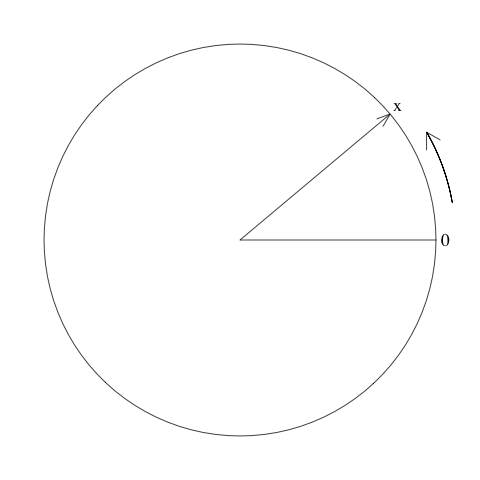
\includegraphics[width=0.5\linewidth]{image/Chap3Spinning.png}
        \caption{轮盘}
        \label{fig:chap03_spining}
    \end{figure}
\end{example}

\begin{remark}
    随机变量$X$本质上是从$(\Omega,\mathcal{F})$到$(R,\mathcal{B})$的可测映射。这里涉及测度论的内容,超出了本课程的内容范围。
\end{remark}

\section{分布函数}

为了掌握随机变量$X$的统计规律,我们只需要掌握$X$的各种取值的概率。由于
\begin{eqnarray*}
    \{a<X\leq b\} &=& \{X\leq b\} - \{X \leq a\};\\
    \{X>c\} &=& \Omega - \{X \leq c\}.
\end{eqnarray*}
因此对于任意实数$x$,只要确定事件$\{X\leq x\}$的概率就可以了。

\begin{definition}{分布函数} \label{def: cdf} 
设$X$为一个随机变量。对任意实数$x$,称
$$
F(x) = P(X\leq x)
$$
为随机变量$X$的{\textbf{累积分布函数}},简称{\textbf{分布函数}}。也称$X$服从$F(x)$,记$X\sim F(x)$。
\end{definition}
\begin{remark}
   任一随机变量$X$都有一个分布函数。
\end{remark}
\begin{problem}
   分布函数的定义是唯一的吗?
\end{problem}
\vspace{3cm}

\begin{property}
任一分布函数$F(x)$都具有如下三条基本性质:
\begin{enumerate}
    \item 单调性:$F(x)$是定义在整个实数轴($-\infty, \infty$)上的单调非减函数,即对任意$x_1 < x_2, F(x_1) \leq F(x_2)$。
    \item 有界性:对任意的$x$,有$0 \leq F(x) \leq 1$,且
 $$\left\{\begin{aligned}
F(-\infty)&=&\lim _{x \rightarrow-\infty} F(x)=0 \\
F(\infty)&=&\lim _{x \rightarrow \infty} F(x)=1
\end{aligned}\right.$$
    \item 右连续性:$F(x)$是$x$的右连续函数,即对任意的$x_0$,
    有
 $$\lim \limits_{x \rightarrow x_0 +0} F(x_0)=0,\quad  F(x_0 + 0=)F(x_0).$$
\end{enumerate}
\end{property}
\begin{proof}
\begin{enumerate}
    \item 设事件$A =\left\{\omega: X(\omega) \leqslant x_{1}\right\} \quad B=\left\{\omega: X(\omega) \leqslant x_{2}\right\}$。若$x_1<x_2$,那么 $A \subset B$。根据概率的单调性,$$P\left(x \leqslant x_{1}\right)=P(A) \leqslant P(B)=P\left(X \leqslant x_{2}\right).$$
    即$F(x_1) \leq F(x_2) $。
    \item 因为 $F(x) = P(X \leq x) $表示事件${X \leq x}$的概率。所以,$0 \leq F(x) \leq 1$。根据$F(x)$的单调性可知,$F(\lfloor x\rfloor) \leqslant F(x) \leqslant F(\lceil x\rceil)$。对于整数$m$和$n$,
  $$ \lim _{x \rightarrow-\infty} F(x)=\lim _{m \rightarrow-\infty} F(m) \quad \lim _{x \rightarrow \infty} F(x)=\lim _{x \rightarrow \infty} F(n) $$
存在。由于概率的可列可加性,
  $$
  \begin{aligned}
1 &=P(-\infty<X<+\infty) \\
&=P\left(\bigcup_{i=-\infty}^{+\infty}\{i-1<X \leqslant i\}\right) \\
&=\sum_{i=-\infty}^{+\infty} P(i-1<X \leqslant i) \\
&=\lim _{n \rightarrow \infty} \lim _{n \rightarrow \infty} \sum_{i=m}^{n} {P(i-1<X \leqslant i)}{}=\lim _{n \rightarrow \infty} \lim _{m \rightarrow-\infty} P(m<X \leqslant n) \\
&=\lim _{n \rightarrow \infty} F(n)-\lim _{m \rightarrow-\infty} F(m) \Rightarrow 1 \geqslant \lim _{n \rightarrow \infty} F(n)=1+\lim _{m \rightarrow \infty} F(m) \geqslant 1 \\
\end{aligned}
  $$
因此,$\lim \limits_{n \rightarrow \infty} F(x)=1=\lim \limits_{x \rightarrow \infty} F(x) \quad ; \lim \limits_{m \rightarrow-\infty} F(m)=0=\lim \limits_{x \rightarrow \infty} F(x)$ 。
\item 因为$F(x)$是有界、单调函数,所以其任一点$x_0$的右极限$F(x_0 +0)$存在。考虑数列 $x_1>x_2>...>x_n>...>x_0$,当$x_n \Rightarrow x_0(n \Rightarrow \infty)$时,
$$\begin{aligned}
F\left(x_{1}\right)-F\left(x_{0}\right) &=P\left(x_{0}<x \leqslant x_{1}\right)=P\left(\bigcup_{i=1}^{\infty}\left\{x_{i+1}<x \leqslant x_{i}\right\}\right) \\
&=\sum_{i=1}^{\infty} P\left(x_{i+1}<x \leqslant x_{i}\right)=\sum_{i=1}^{\infty} F\left(x_{i}\right)-F\left(x_{i+1}\right) \\
&=\lim _{n \rightarrow \infty} \sum_{i=1}^{n}\left[F\left(x_{i}\right)-F\left(x_{i+1}\right)\right]=F\left(x_{1}\right)-\lim _{n \rightarrow \infty} F\left(x_{n}\right) \\
\end{aligned}$$
因此,$F\left(x_{0}\right) =\lim _{n \rightarrow \infty} F\left(x_{n}\right)=F\left(x_{0}+0\right)$。
\end{enumerate}
\end{proof}
\begin{remark}
    \begin{enumerate}
        \item 这三条基本性质也是判断某个函数是否为某个随机变量的分布函数的充要条件。
        \item 利用分布函数,我们可以容易地计算概率
        \begin{itemize}
            \item $P(X>x) = 1-F(x)$;
            \item $P(X<x) = F(x-0) = \lim_{y\rightarrow x-} F(y)$;
            \item $P(X=x) = F(x)-F(x-0)$;
            \item $P(X\geq x) = 1- F(x-0)$;
            \item $P(a< X\leq b) =F(b)-F(a)$;
            \item $P(a<X<b) = F(b-0)-F(a)$;
            \item $P(a\leq X<b) = F(b-0) - F(a-0)$;
            \item $P(a\leq X\leq b) = F(b) - F(a-0)$。
        \end{itemize}
        \item 特别地,$F(x)$在a,b处连续时,有$F(a-0) = F(a)$且$F(b-0) =F(b)$。
    \end{enumerate}
\end{remark}
\begin{example}
    对于反正切函数
$$F(x)=\frac{1}{\pi}\left(\arctan x+\frac{\pi}{2}\right),-\infty<x<\infty.$$
我们可以发现
\begin{enumerate}
    \item $F(x)$是连续且严格单调增函数;
    \item $F(\infty) = 1$ 且 $F(-\infty) = 0$;
    \item $F(x)$是某个随机变量的分布函数,该分布为柯西分布。
    \item 设$X$为一个服从柯西分布的随机变量,则
    \begin{eqnarray*}
        P(-1\leq X \leq 1) &=& F(1) - F(-1) \\&=& \frac{1}{\pi}\left(\arctan(1) - \arctan(-1)\right)\\
        &=&\frac{1}{2}.
    \end{eqnarray*}
\end{enumerate}
\end{example}

\section{分位数}
除了期望的特征数之外,分位数是随机变量及其分布的另一类特征数。

\begin{definition}\label{def:quantile}
设连续随机变量$X$的分布函数为$F(x)$,密度函数为$p(x)$。对任意$ p \in(0,1),$,称满足条件
$$F\left(x_{p}\right)=\int_{-\infty}^{x_{p}} p(x) d x=p$$
的$x_{p}$为此分布的$p$分位数,又称下侧$p$分位数。

称满足条件
$$1-F\left(x_{p}^{\prime}\right)=\int_{x_{p}^{\prime}}^{+\infty} p(x) d x=p$$
的$x_{p}^{\prime}$为此分布的上侧$p$分位数。
\end{definition}


\begin{definition}
设连续随机变量$X$的分布函数为$F(x)$,密度函数为$p(x)$,称$p=0.5$时的$p$分位数$x_{0.5}$为此分布的中位数,即
$$F\left(x_{0.5}\right)=\int_{-\infty}^{x_{0.5}} p(x) d x=0.5$$
\end{definition}

\begin{example}
    若$X$服从参数为$\lambda$的指数分布,求其中位数。
\end{example}
\begin{solution}
    $X$的分布函数为
    $$
    F(x) = 1 - \exp\{-\lambda x\}.
    $$
    设$x_{0.5}$为所求的中位数,即
    $$F(x_{0.5}) =  1 - \exp\{-\lambda x_{0.5}\} = 0.5.$$
    则
    $$
    x_{0.5} = \ln(2)/\lambda.
    $$
\end{solution}

\section{习题}

    \begin{enumerate}


\item 设随机变量$X$服从双参数韦布尔分布,其分布函数为
$$
	    F(x) = 1-\exp \left \{-\left (\frac{x}{\eta} \right )^m \right \}, x>0,
$$
其中$\eta > 0,m > 0$.试写出该分布的$p$分位数$x_p$的表达式,且求出当$m = 1.5,\eta = 1000$时的$x_{0.1},x_{0.5},x_{0.8}$的值。

\end{enumerate}